% Tikz File 'flowchart.tex'
\documentclass{standalone}
\usepackage{tikz}
\usetikzlibrary{shapes.geometric, arrows}

  
    \tikzstyle{node} = [rectangle, rounded corners, minimum width=3cm, minimum height=1cm,text width = 4 cm,text centered, draw=black, fill=red!30]
    \tikzstyle{io} = [trapezium, trapezium left angle=70, trapezium right angle=110, text width = 4cm,minimum width=1cm,minimum height=1cm, text centered, draw=black, fill=blue!30]
    \tikzstyle{io1} = [trapezium, trapezium left angle=70, trapezium right angle=110, minimum width=1cm,minimum height=1cm, text centered, draw=black, fill=blue!30]
    \tikzstyle{process} = [rectangle, minimum width=3cm, minimum height=1cm,text width = 4cm,text centered, draw=black, fill=orange!30]
    \tikzstyle{decision} = [diamond, minimum width=3cm, minimum height=1cm,text width = 2cm,text centered, draw=black, fill=green!30]    
    \tikzstyle{arrow} = [thick,->,>=stealth]


\begin{document}
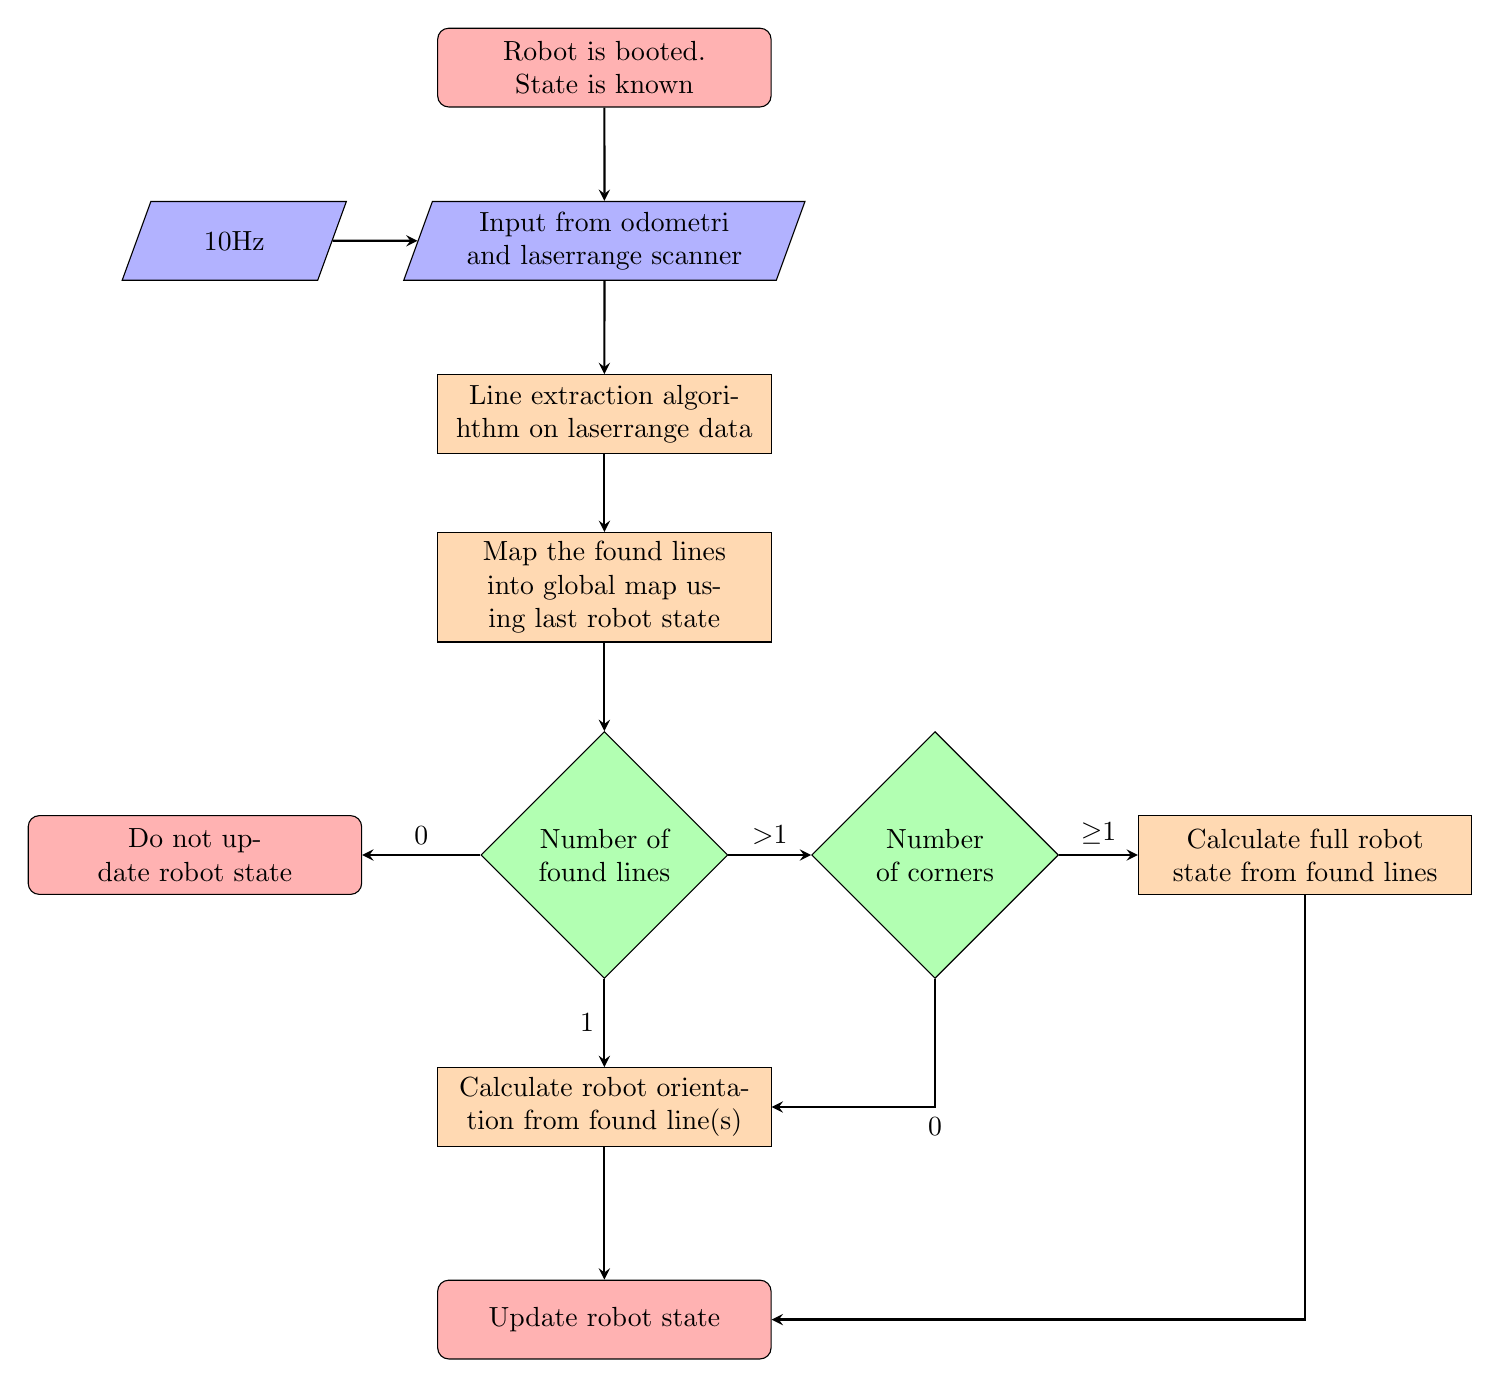
\begin{tikzpicture}[node distance=2.2cm]

%% NODES
\node (start) [node] {Robot is booted.  State is known};
\node (input) [io, below of=start] { Input from odometri and laserrange scanner };
\node (input1) [io1, left of=input, xshift=-2.5cm] {10Hz };
\node (pro1) [process, below of=input] {Line extraction algorihthm on laserrange data};
\node (pro2) [process, below of=pro1] {Map the found lines into global map using last robot state};
\node (dec1) [decision, below of =pro2, yshift=-1.2cm] {Number of found lines};
\node (pro4) [node, left of=dec1, xshift = -3cm ] {Do not update robot state};
\node (pro5) [process, below of=dec1, yshift = -1cm ] {Calculate robot orientation from found line(s)};
\node (pro6) [node, below of=pro5,yshift =-0.5cm] {Update robot state};
\node (dec2) [decision,right of= dec1, xshift =2cm] {Number of corners};
\node (pro3) [process, right of =dec2, xshift = 2.5cm ] {Calculate full robot state from found lines};



%% ARROWS
\draw [arrow] (start) -- (input);
\draw [arrow] (input) -- (pro1);
\draw [arrow] (pro1) -- (pro2);
\draw [arrow] (pro2) -- (dec1);
\draw [arrow] (dec1) -- node[anchor=south] {\textgreater1} (dec2);
\draw [arrow] (dec1) -- node[anchor=south] {0} (pro4);
\draw [arrow] (dec1) -- node[anchor=east] {1} (pro5);
\draw [arrow] (pro5) -- (pro6);
\draw [arrow] (pro3) |- (pro6);
\draw [arrow] (input1) -- (input);
\draw [arrow] (dec2) |- node[anchor=north] {0}(pro5);
\draw [arrow] (dec2) -- node[anchor=south] {$\geq$1} (pro3);
\end{tikzpicture}
\end{document}